\section{Ordered densities of squared singular values of a Gaussian matrix product}

This rather simple result is a humble acknowledgement of the great work in finite-size random matrix theory (RMT) by Prof. Gernot Akemann and team at Uni Bielefeld. For finding the ordered densities, a straightforward recursive formulation, in terms of the MeijerG function, based on the work of Alberto Zanella at CNR in Italy, is utilized.

Note: Several integration formulas for the MeijerG function are known, e.g., see the MeijerG function reference.
Although the expressions are complex, they can be numerically evaluated quite easily via Mathematica or MATLAB. It amazes me that these finite-size RMT densities are even analytically approachable, although, undoubtedly, the asymptotic RMT theory is "more elegant."

The theorem is as follows. See below for Mathematica code and numerical simulations.

Theorem

\begin{figure}[H]
	\centering
	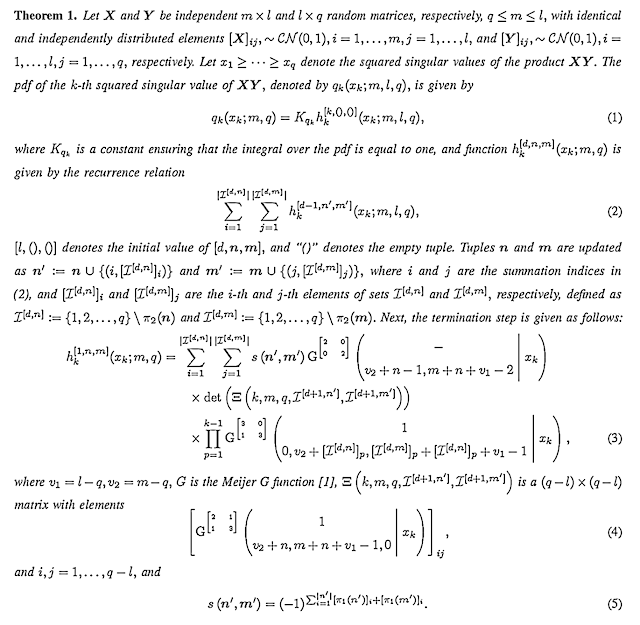
\includegraphics[width=0.5\textwidth,keepaspectratio]{015_001_1-Theorem.png}
\end{figure}

Second projection notation: Let set $s := \{(1,2), (3,4), (5,6)\}$ be a set containing three tuples. Then, $\pi_2(s)$ is the second projection of $s$ given by $\pi_2(s) = \{2, 4, 6\}.$

Proof

Below, a sketch of the proof for completeness.

\begin{figure}[H]
	\centering
	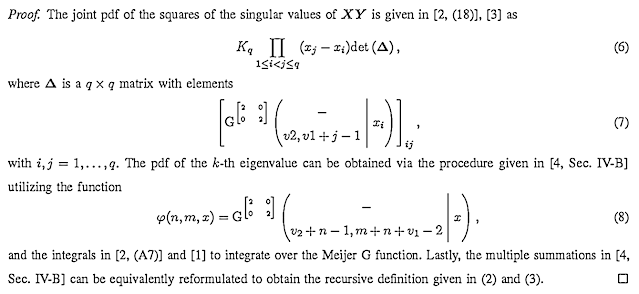
\includegraphics[width=0.5\textwidth,keepaspectratio]{015_002_1-Proof.png}
\end{figure}
\begin{figure}[H]
	\centering
	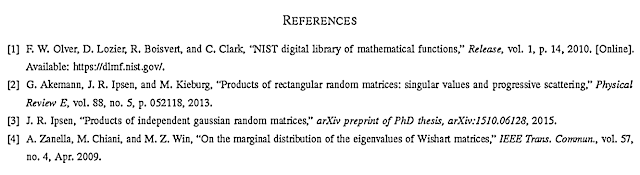
\includegraphics[width=0.5\textwidth,keepaspectratio]{015_003_1-References.png}
\end{figure}

Mathematica Code

Now, a Mathematica package for evaluating the ordered densities is as follows. Here, in $xyz[symb_, l, v_2, v_1, q_],$ $symb$ is the desired symbol for the variable, e.g., $x,$ $l$ is the index (corresponding to $k$ in the theorem), $v_1, v_2,$ and $q$ are as in the theorem above.

\begin{verbatim}
(* ::Package:: *)

BeginPackage["xyl`"]
(*** Exported Symbol ***)
xyl
Begin["`Private`"]

\[CurlyPhi][v2_, v1_, q_, n_, m_] := MeijerG[{{}, {}}, {{v2+n-1, m + n+v1 - 2}, {}}, s]; 
Iup[v2_, v1_, q_, n_, m_] := MeijerG[{{}, {1}}, {{0, v2+n, m + n+v1 - 1}, {}}, s]; 
Idown[v2_, v1_, q_, n_, m_] := MeijerG[{{1}, {}}, {{v2+n, m + n+v1 -1}, {0}}, s]; 
r[i_, n_, q_] := Complement[Range[q], n][[i]]
sg[n_, m_, q_] := Product[(-1)^(FirstPosition[Complement[Range[q], m[[1 ;; i - 1]]], m[[i]]] + FirstPosition[Complement[Range[q], n[[1 ;; i - 1]]], n[[i]]]), {i, 1, Length[n]}]
Dmat[l_, v2_, v1_, q_, ns_, ms_] := Piecewise[{{1, l == q}}, Det[Table[Idown[v2, v1, q, r[n, ns, q], r[m, ms, q]], {n, 1, q - l}, {m, 1, q - l}]]]
xylpdf[l_, v2_, v1_, q_, d_, ns_, ms_] := Sum[xylpdf[l, v2, v1, q, d - 1, Append[ns, n], Append[ms, m]], {n, Complement[Range[q], ns]}, {m, Complement[Range[q], ms]}]
xylpdf[l_, v2_, v1_, q_] := xylpdf[l, v2, v1, q, l, {}, {}]
xylpdf[l_, v2_, v1_, q_, 1, ns_, ms_] := Product[Iup[v2, v1, q, ns[[i]], ms[[i]]], {i, 1, l - 1}]*
Sum[\[CurlyPhi][v2, v1, q, n, m]*sg[Append[ns, n], Append[ms, m], q]*Dmat[l, v2, v1, q, Append[ns, n], Append[ms, m]], {n, Complement[Range[q], ns]}, {m, Complement[Range[q], ms]}]
xyl[symb_,l_?NumericQ,v2_?NumericQ,v1_?NumericQ,q_?NumericQ] := xylpdf[l, v2, v1, q]/(Product[Gamma[n] Gamma[n+v1] Gamma[n+v2],{n,1,q}] Factorial[l-1]) /. s->symb ;

End []
EndPackage[]
\end{verbatim}

Numerical Results

Lastly, the numerical simulations for $v_1 = 6, v_2 = 2,$ and $q = 2.$ We see that the results based on the above expressions and those based on Monte-Carlo simulations agree well.

\begin{figure}[H]
	\centering
	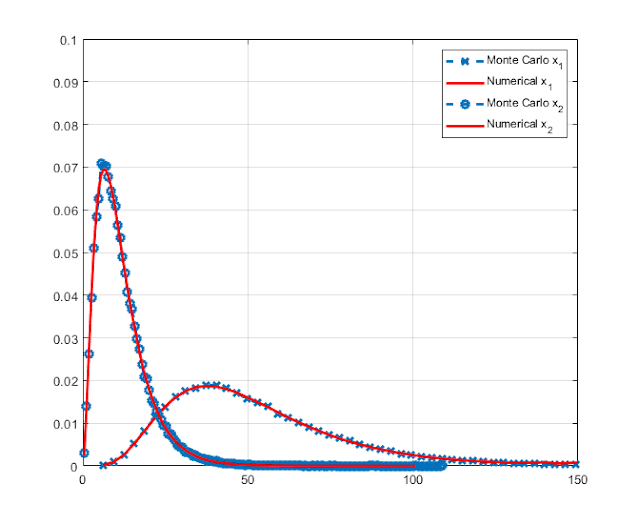
\includegraphics[width=0.5\textwidth,keepaspectratio]{015_004_1.png}
\end{figure}

- ARK

\emph{First published: 9th Jul. 2022 on aravindhk-math.blogspot.com}
